\documentclass[handout]{beamer}
\usepackage{graphicx} % Required for inserting images
% \usepackage[latin2]{inputenc}
\usepackage{amsmath}
\usepackage{mathtools}
\usepackage[shortlabels]{enumitem} % for {enumerate}[a]
%\usepackage[pdftex]{graphicx}
\usepackage{amsfonts}
\usepackage{amssymb}
%\usepackage{fancyhdr}
\usetheme{Madrid}
%\pagestyle{fancyplain}
\usepackage{mathrsfs}  
\usepackage{setspace}
\usepackage{epsfig}
\usepackage{color}
\usepackage{tikz}
%\usepackage{UVMThesisStyle-July2020}
%\usepackage{cancel}
\usepackage{float}
%\usepackage{cite}
\usepackage{url}


%my own packages
\usepackage{latexsym}
\usepackage{amssymb}
\usepackage{amsthm}
\usepackage{amscd}
\usepackage{amsmath}
\usepackage{tikz-cd}
\usepackage{soul}
\usepackage{subfiles}


%theorem style commands
%\newtheorem{theorem}{Theorem}[section]
%\newtheorem{fact}[theorem]{Fact}
%\newtheorem{claim}[theorem]{Claim}
%\newtheorem{lemma}[theorem]{Lemma}
%\newtheorem{definition}[theorem]{Definition}
%\newtheorem{proposition}[theorem]{Proposition}
%\newtheorem{corollary}[theorem]{Corollary}
%\newtheorem{conjecture}[theorem]{Conjecture}
%\newtheorem{hypothesis}[theorem]{Hypothesis}
%\newtheorem{example}[theorem]{Example}
%\newtheorem{remark}[theorem]{Remark}


%\theoremstyle{remark}
\newtheorem{case}{Case}

\numberwithin{equation}{section}
\numberwithin{case}{theorem}

%shortcuts
\newcommand{\cA}{\mathcal{A}}		%curly a
\newcommand{\cB}{\mathcal{B}}		%curly b
\newcommand{\cC}{\mathcal{C}}		%curly c
\newcommand{\cD}{\mathcal{D}}		%curly d
\newcommand{\cE}{\mathcal{E}}		%curly e
\newcommand{\cF}{\mathcal{F}}		%curly f
\newcommand{\cG}{\mathcal{G}}		%curly g
\newcommand{\cH}{\mathcal{H}}		%curly h
\newcommand{\cI}{\mathcal{I}}		%curly i
\newcommand{\cJ}{\mathcal{J}}		%curly j
\newcommand{\cK}{\mathcal{K}}		%curly k
\newcommand{\cL}{\mathcal{L}}		%curly l
\newcommand{\cM}{\mathcal{M}}		%curly m
\newcommand{\cN}{\mathcal{N}}		%curly n
\newcommand{\cO}{\mathcal{O}}		%curly o
\newcommand{\cP}{\mathcal{P}}		%curly p
\newcommand{\cQ}{\mathcal{Q}}		%curly q
\newcommand{\cR}{\mathcal{R}}		%curly r
\newcommand{\cS}{\mathcal{S}}		%curly s
\newcommand{\cT}{\mathcal{T}}		%curly t
\newcommand{\cU}{\mathcal{U}}		%curly u
\newcommand{\cV}{\mathcal{V}}		%curly v
\newcommand{\cW}{\mathcal{W}}		%curly w
\newcommand{\cX}{\mathcal{X}}		%curly x
\newcommand{\cY}{\mathcal{Y}}		%curly y
\newcommand{\cZ}{\mathcal{Z}}		%curly z

\newcommand{\sA}{\mathscr{A}}		%script a
\newcommand{\sB}{\mathscr{B}}		%script b
\newcommand{\sC}{\mathscr{C}}		%script c
\newcommand{\sD}{\mathscr{D}}		%script d
\newcommand{\sE}{\mathscr{E}}		%script e
\newcommand{\sF}{\mathscr{F}}		%script f
\newcommand{\sG}{\mathscr{G}}		%script g
\newcommand{\sH}{\mathscr{H}}		%script h
\newcommand{\sI}{\mathscr{I}}		%script i
\newcommand{\sJ}{\mathscr{J}}		%script j
\newcommand{\sK}{\mathscr{K}}		%script k
\newcommand{\sL}{\mathscr{L}}		%script l
\newcommand{\sM}{\mathscr{M}}		%script m
\newcommand{\sN}{\mathscr{N}}		%script n
\newcommand{\sO}{\mathscr{O}}		%script o
\newcommand{\sP}{\mathscr{P}}		%script p
\newcommand{\sQ}{\mathscr{Q}}		%script q
\newcommand{\sR}{\mathscr{R}}		%script r
\newcommand{\sS}{\mathscr{S}}		%script s
\newcommand{\sT}{\mathscr{T}}		%script t
\newcommand{\sU}{\mathscr{U}}		%script u
\newcommand{\sV}{\mathscr{V}}		%script v
\newcommand{\sW}{\mathscr{W}}		%script w
\newcommand{\sX}{\mathscr{X}}		%script x
\newcommand{\sY}{\mathscr{Y}}		%script y
\newcommand{\sZ}{\mathscr{Z}}		%script z

\newcommand{\bbA}{\mathbb{A}}		%bold a
\newcommand{\bbB}{\mathbb{B}}		%bold b
\newcommand{\bbC}{\mathbb{C}}		%bold c
\newcommand{\bbD}{\mathbb{D}}		%bold d
\newcommand{\bbE}{\mathbb{E}}		%bold e
\newcommand{\bbF}{\mathbb{F}}		%bold f
\newcommand{\bbG}{\mathbb{G}}		%bold g
\newcommand{\bbH}{\mathbb{H}}		%bold h
\newcommand{\bbI}{\mathbb{I}}		%bold i
\newcommand{\bbJ}{\mathbb{J}}		%bold j
\newcommand{\bbK}{\mathbb{K}}		%bold k
\newcommand{\bbL}{\mathbb{L}}		%bold l
\newcommand{\bbM}{\mathbb{M}}		%bold m
\newcommand{\bbN}{\mathbb{N}}		%bold n
\newcommand{\bbO}{\mathbb{O}}		%bold o
\newcommand{\bbP}{\mathbb{P}}		%bold p
\newcommand{\bbQ}{\mathbb{Q}}		%bold q
\newcommand{\bbR}{\mathbb{R}}		%bold r
\newcommand{\bbS}{\mathbb{S}}		%bold s
\newcommand{\bbT}{\mathbb{T}}		%bold t
\newcommand{\bbU}{\mathbb{U}}		%bold u
\newcommand{\bbV}{\mathbb{V}}		%bold v
\newcommand{\bbW}{\mathbb{W}}		%bold w
\newcommand{\bbX}{\mathbb{X}}		%bold x
\newcommand{\bbY}{\mathbb{Y}}		%bold y
\newcommand{\bbZ}{\mathbb{Z}}		%bold z

\newcommand{\rI}{\mathrm{I}}
\newcommand{\rII}{\mathrm{II}}


\newcommand{\Proj}{\operatorname{Proj}} 	%Proj
\newcommand{\sProj}{\operatorname{sProj}} 	%sProj
\newcommand{\res}{\mathrm{res}} 	%res
\newcommand{\Hom}{\operatorname{Hom}} 	%Hom
\newcommand{\GL}{\mathrm{GL}} 	%GL
\newcommand{\PGL}{\mathrm{PGL}} 	%PGL
\newcommand{\PSL}{\mathrm{PSL}} 	%SGL
\newcommand{\SL}{\mathrm{SL}} 	%SL
\newcommand{\Frob}{\mathrm{Frob}} 	%Frob
\newcommand{\Isom}{\mathrm{Isom}} 	%Isom
\newcommand{\Span}{\mathrm{Span}} 	%Span
\newcommand{\Aut}{\mathrm{Aut}} 	%Aut
\newcommand{\End}{\mathrm{End}} 	%End
\newcommand{\Gal}{\mathrm{Gal}} 	%Gal
\newcommand{\Ring}{\mathrm{Ring}} 	%Ring
\newcommand{\AbGrp}{\mathrm{AbGrp}} 	%AbGrp
\newcommand{\Cring}{\mathrm{CRing}} 	%CRing
\newcommand{\Sym}{\operatorname{Sym}} 	%Sym
\newcommand{\coker}{\mathrm{coker}} 	%coker
\newcommand{\Spec}{\operatorname{Spec}} %Spec
\newcommand{\Jac}{\operatorname{Jac}} 	%Jac
\renewcommand{\div}{\operatorname{div}} % divisor of a function
\newcommand{\ord}{\operatorname{ord}}   % order of a function at a point
\newcommand{\MD}{\operatorname{MD}} 	% minimal decomposition

% Frequently used math commands
\newcommand{\vep}{\varepsilon}
\newcommand{\union}{\cup}
\newcommand{\intsec}{\cap}
\newcommand{\cross}{\times}
\newcommand{\tensor}{\otimes}
\newcommand{\floor}[1]{\lfloor #1 \rfloor}
\newcommand{\ceil}[1]{\lceil #1 \rceil}
\newcommand{\Floor}[1]{\left\lfloor #1 \right\rfloor}
\newcommand{\Ceil}[1]{\left\lceil #1 \right\rceil}
\newcommand{\size}[1]{\lvert #1 \rvert}
\newcommand{\Size}[1]{\left\lvert #1 \right\rvert}
\newcommand{\textand}{\quad \text{and} \quad}
\newcommand{\textor}{\quad \text{or} \quad}
\newcommand{\<}{\left\langle}
\renewcommand{\>}{\right\rangle}
\newcommand{\ignore}[1]{}
\newcommand{\Mod}[1]{\ (\mathrm{mod}\ #1)}
% 
\newcommand{\ib}{{\text{\ref*{it:ord2}}}}
\newcommand{\ic}{{\text{\ref*{it:ord3}}}}
\newcommand{\id}{{\text{\ref*{it:c1+c2}}}}

% For diagrams
\setlength{\unitlength}{0.5cm}
\newcommand{\solid}[1]{\put#1{\circle*{0.25}}}
\newcommand{\open}[1]{\put#1{\circle{0.25}}}
\newcommand{\xdot}[1]{\put#1{\makebox(0,0){\small +}}}

\newcommand{\jesse}[1]{{\color{blue} \sf $\spadesuit\spadesuit\spadesuit$ Jesse: [#1]}} %editorial comments
\newcommand{\todo}[1]{{\color{red} \sf $\spadesuit\spadesuit\spadesuit$ TODO: [#1]}}

%footer setup
\makeatother
\setbeamertemplate{footline}
{
	\leavevmode%
	\hbox{%
		\begin{beamercolorbox}[wd=.4\paperwidth,ht=2.25ex,dp=1ex,center]{author in head/foot}%
			\usebeamerfont{author in head/foot}\insertshortauthor
		\end{beamercolorbox}%
		\begin{beamercolorbox}[wd=.6\paperwidth,ht=2.25ex,dp=1ex,center]{title in head/foot}%
			\usebeamerfont{title in head/foot}\insertshorttitle\hspace*{3em}
			\insertframenumber{} / \inserttotalframenumber\hspace*{1ex}
	\end{beamercolorbox}}%
	\vskip0pt%
}
\makeatletter
\setbeamertemplate{navigation symbols}{}


\title{Geometry of Drinfeld Modular Forms}
\author{Jesse Franklin}
\institute{University of Vermont}
\date{Workshop on Number Theory in Function Fields\\at Penn State, $2024$}



\begin{document}
	
	\frame{\titlepage}
	
	\begin{frame}
		\frametitle{Notation}
		$q$ - a power of an odd prime.\\ 
		$K$ - the function field of some smooth, connected, projective curve over a field of characteristic $q,$ \pause  e.g.\ $\bbP^1$
		
		\[\begin{array}{ccl}
			\text{Classical Setting} && \text{Function Field}\\
			\hline
			\bbZ && A\overset{def}{=}\bbF_q[T]\pause\\
			\bbQ && K \overset{def}{=} \bbF_q(T)\pause\\
			\bbR && K_{\infty}\overset{def}{=}\bbF_q\left(\!\left(\frac{1}{T}\right)\!\right) \pause\\
			\bbC && C \overset{def}{=} \widehat{\overline{K_{\infty}}}\pause\\
			\cH = \{a+bi\in \bbC:b>0\} && \Omega \overset{def}{=} C-K_{\infty}\pause\\
			\SL_2(\bbZ)\setminus\cH && \GL_2(A)\setminus \Omega\\
			&\left(\begin{array}{cc}a&b\\c&d\end{array}\right)z=\frac{az+b}{cz+d}&
		\end{array}\]
	\end{frame}
	
	\begin{frame}
		\frametitle{The classical thing we want to analogize}
		Let $\Gamma\leq \PSL_2(\bbR)$ be a Fuchsian group with finite coarea. Let $\sX(\Gamma)$ denote the stacky curve over $\bbC$ which is the algebraization of the compactified orbifold quotient $X=\Gamma\setminus \cH^{(*)}.$ \pause We know (e.g.\ \cite[Chapter $6$]{VZB})
		\begin{align*}
			M(\Gamma)\overset{def}{:=}\bigoplus_{k\geq 0}M_k(\Gamma)&\overset{\sim}{\longrightarrow} \bigoplus_{k\geq 0} H^0(\sX_{\Gamma},\Omega^1_{\sX_{\Gamma}}(\Delta)^{\otimes k/2})\overset{def}{=:}R(\sX_{\Gamma};\Delta),\\
			&f\mapsto fdz^{\otimes k/2}
		\end{align*}
		
		\pause 

		\cite[page $13$]{Gekeler-Curves}:
		\includegraphics[scale=0.45]{gek-pg13.png}
	\end{frame}	
	
	\begin{frame}
		\frametitle{Why Stacks? What are Stacks?}
		Modular forms are *always* sections of a line bundle.\\ \pause
		However, \[H^0(X,L^{\otimes k})\neq M_k(\Gamma)\quad\quad \text{ and }\quad\quad R(X;L)\neq M(\Gamma),\] 
		where
		\[\begin{cases}
			X &= \text{moduli scheme},\\ 
			L &= \text{appropriate line bundle},\\
			M &= \text{vector space of modular forms}.
		\end{cases}\] \pause
		
		So, \textbf{what are stacks?} \pause
		\[\begin{array}{c|c}
			1\text{-category}&2\text{-category}\\ 
			\hline
			\text{functor / pre-sheaf}&\text{fibered category}\\ 
			\text{separated pre-sheaf}&\text{pre-stack}\\ 
			\text{sheaf}&\text{stack}\\ 
			\text{algebraic space / scheme}&\text{algebraic stack}\\
			\text{variety}&\text{algebraic stack of finite type over a field}
		\end{array}\]
	\end{frame}
	
	\begin{frame}
		\frametitle{So, what are stacks?}
			\begin{definition}%[{\cite[$2.1$]{Landesman-Ruhm-Zhang-Spin-canonical-rings}}]
				A \textbf{stacky curve} over an algebraically closed field $\bbK$ is:
				\begin{itemize}
					\item[$\cdot$] a smooth, integral, proper, scheme $X$ of dimension $1$, together with\\ \pause
					\item[$\cdot$] a finite number of closed points $P_1,\ldots, P_r$ called \textbf{stacky points} with stabilizer orders $e_1,\ldots, e_r\in \bbZ_{\geq 2}.$
				\end{itemize}
			\end{definition}
			\pause
			\begin{example}[{\cite[Corollary $1.4.3$]{Laumon-cohomology-Drinfeld-modular-varieties}}]
				The moduli space $\cM^2_A$ of rank $2$ Drinfeld modules with no level structure is known to be a Deligne-Mumford algebraic stack of finite type over $\bbF_p.$ 
			\end{example}
	\end{frame}	
	
	\begin{frame}
		\frametitle{Stacky Curves $101$}		
			Let $\sX$ denote a stacky curve with \textbf{signature} $\sigma=(g;e_1,\ldots, e_r).$ \pause
			We say that $D\in \operatorname{Div}(\sX)$ has
			\[\deg(D)=\lfloor D\rfloor=\Big\lfloor\sum_ia_iP_i\Big\rfloor\overset{def}{=}\sum_i \floor{a_i}\pi(P_i),\]
			where $\pi:\sX\to X$ is the coarse space morphism. \pause The \textbf{(log) canonical ring of $(\sX; \Delta)$} is 
			\[R(\sX;\Delta)=\bigoplus_{d\geq 0} H^0(\sX,d(K_{\sX}+\Delta)),\]
			where \[K_{\sX}\sim K_X+\left(\sum_{i=1}^r \frac{1}{e_i}P_i\right),\] is a \textbf{canonical divisor} of $\sX$ and $\Delta=\sum_jQ_j\in \operatorname{Div}(\sX)$ is a \textbf{log divisor}. 
	\end{frame}	
	
	\begin{frame}
		\frametitle{Computing the Canonical Ring of a Stacky Curve}
		\cite{VZB} gives an inductive presentation of $R(\sX)$ for $\sX$ with $\sigma=(g;e_1,\ldots, e_r)$ in terms of $R(\sX')$ with $\sigma'=(g;e_1,\ldots, e_{r-1})$: \pause
		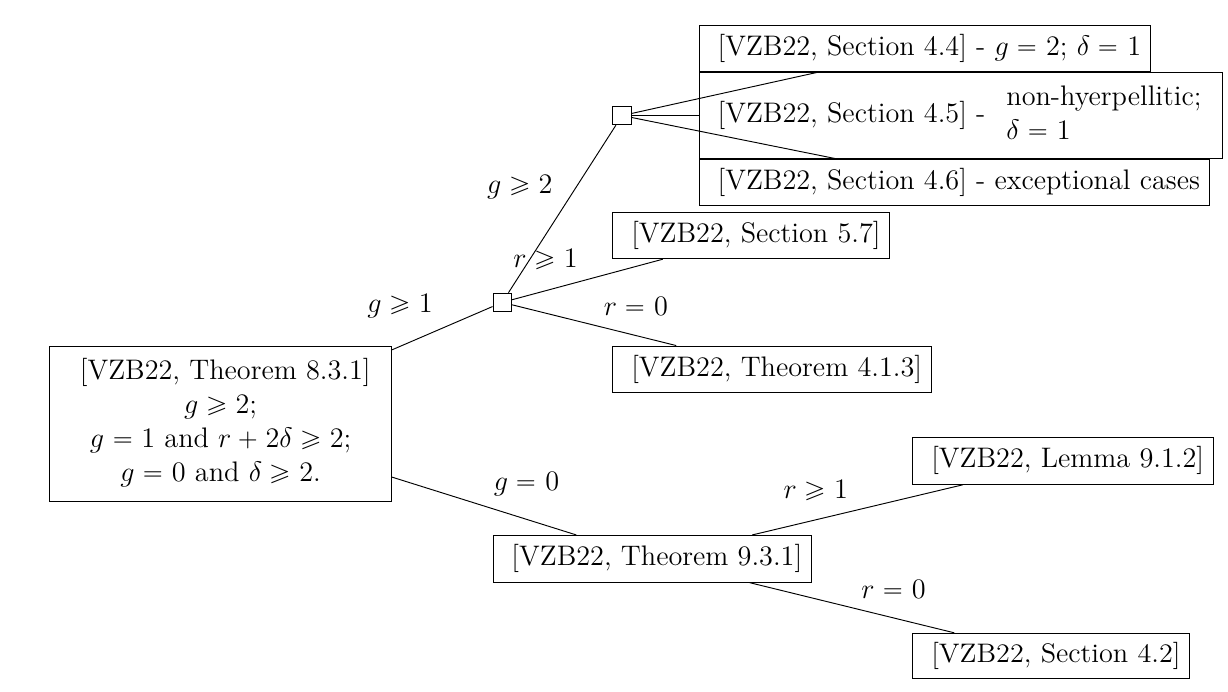
\includegraphics[scale=0.5]{VZB.png}
	\end{frame}
	
	\begin{frame}
		\frametitle{Old Friends}
		\begin{example}[Goss and Gekeler's famous $\GL_2(A)$-forms]
			\begin{itemize}
				\item[$\cdot$] $g$ of weight $q-1$ and type $0,$ \pause 
				\item[$\cdot$] $\Delta$ of weight $q^2-1$ and type $0,$ \pause 
				\item[$\cdot$] $h$ of weight $q+1$ and type $1.$ \pause 
			\end{itemize}
			\pause
			\[\bigoplus_{k\geq 0} M_{k,0}(\GL_2(A))=C[g,\Delta] \quad \text{and}\quad \bigoplus_{\substack{k\geq 0\\l\Mod{q-1}}} M_{k,l}(\GL_2(A))=C[g,h].\]
		\end{example}
		
		\pause
		
		\begin{example}[Stacky $j$-line]
			$\sX_{\GL_2(A)}\cong \bbP^1(q-1,q+1)$ is a \textbf{football} (see e.g.\ \cite[$5.3.14$]{VZB}):\\ \pause \quad\quad\quad\quad\quad\quad\quad\quad\quad\quad
			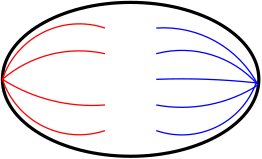
\includegraphics[scale=0.25]{football.png}\\
			\pause
			\textbf{But,} $R(\sX_{\GL_2(A)})\neq C[g,h].$
		\end{example}
	\end{frame}
	
	\begin{frame}
		\frametitle{What goes ``Wrong'' in Function Fields}		
		Among other resources, we have: 
		\[\begin{cases}
				\text{\cite{Gekeler-Invariants}} & \text{for signatures of Drinfeld modular curves, and}\\
				\text{\cite{VZB}} & \text{for computing canonical rings of stacky curves.}
			\end{cases}
		\]
		
		\pause 
		So, \textbf{where's our modular forms $=$ sections of a line bundle?} \pause 
	
		We will consider:
		\begin{itemize}
			\item[$\cdot$] weight and type of Drinfeld modular forms; \pause
			\item[$\cdot$] exponentials and $u$-series; \pause
			\item[$\cdot$] special congruence groups $\Gamma\leq \GL_2(A)$; \pause
			\item[$\cdot$] elliptic points and cusps of Drinfeld modular curves; \pause
			\item[$\cdot$] GAGA for rigid analytic stacks.
		\end{itemize}
	\end{frame}	
	
	\begin{frame}
		\frametitle{Drinfeld Modular Forms}
		\begin{definition}%[{\cite[$(3.1)$]{Gekeler-Curves}}]
			Let $\Gamma\leq \GL_2(A)$ be a congruence subgroup. A \textbf{modular form} of \textbf{weight} $k\in \bbZ_{\geq0}$ and \textbf{type} $l\in \bbZ/((q-1) \bbZ)$ is a map $f:\Omega\to C$ such that\pause 
			\begin{itemize}
				\item[$1.$] $f$ is holomorphic on $\Omega$ and at the cusps of $\Gamma$; \pause
				\item[$2.$] $f(\gamma z)=\det(\gamma)^{-l}(cz+d)^kf(z)$ for all $\gamma=\begin{psmallmatrix}a&b\\c&d\end{psmallmatrix}\in \Gamma.$
			\end{itemize}
		\end{definition}
		
		\pause
		\begin{lemma}[{\cite[Remark $(5.8.\mathrm{i})$]{Gekeler-Coeff}}]\label{l: weight-type}
			If $M_{k,l}(\Gamma)\neq 0,$ then $k\equiv 2l\pmod{q-1}.$
		\end{lemma}
		\pause
		\begin{proof}
			If $f$ is non-zero modular for $\Gamma$ of weight $k$ and type $l$ then \[f(\begin{psmallmatrix}\alpha&0\\0&\alpha\end{psmallmatrix}z)=f\left(\frac{\alpha z}{\alpha}\right)=f(z)=\alpha^k\alpha^{-2l}f(z).\]
		\end{proof}
	\end{frame}
	
	\begin{frame}
		\frametitle{``Fourier series'' for Drinfeld Modular Forms}
		\begin{definition}\label{d: parameter at infty}
			We define a \textbf{parameter at infinity} 
			\[u(z)\overset{def}{=}\frac{1}{e_{\overline{\pi}A}(\bar{\pi}z)}=\frac{1}{\bar{\pi}e_A(z)}=\bar{\pi}^{-1}\sum_{a\in A}\frac{1}{z+a}.\]
			
			\pause 
			
			Recall:
			\begin{itemize}
				\item[$\cdot$] $\displaystyle{u\left(\alpha z\right)=\alpha^{-1}u(z)}$ for any $\alpha\in \bbF_q^{\times}.$ \pause
				\item[$\cdot$] $u$-series coefficients for a Drinfeld modular form uniquely determine the form. 
			\end{itemize}
		\end{definition}
		
		%\pause
		%\begin{lemma}[{\cite[Remark $5.8.\mathrm{iii}$]{Gekeler-Coeff}}]\label{l: u-series coeffs determine form}
		%	Suppose $f(z)\in M_{k,l}(\Gamma)$ has a $u$-series expansion $\displaystyle{f(z)=\sum_{n\geq 0}a_nu^n.}$ Then \emph{the coefficients $a_i$ uniquely determine $f.$}
		%\end{lemma}
		
		\pause 
		\begin{lemma}
			$\displaystyle{\frac{de_A(z)}{dz}=1\Rightarrow \frac{du}{u^2} = -\overline{\pi}dz,}$ i.e.\ the differential $dz$ has a double pole at $\infty.$
		\end{lemma}
	\end{frame}
	
	\begin{frame}
		\frametitle{From Florian and Gebhard with Love}
			Drinfeld modular forms are \emph{sensitive to determinants}, so consider some ``friendlier'' modular forms for Breuer and B\"ockle's special congruence subgroups:\pause
			
			\begin{itemize}
			 	\item[]\cite{Breuer-Gekeler-h-function} Let $\Gamma_2\overset{def}{=}\{\gamma\in \Gamma:\det(\gamma)\in (\det\Gamma)^2\}.$\\ \quad (Suppose $\det\Gamma_2=(\bbF_q^{\times})^2.$) \pause
			 	\item[][B\"ockle] Let $\Gamma_1\overset{def}{=}\{\gamma\in \Gamma: \det(\gamma)=1\}.$ Suppose $\Gamma'$ is such that $\Gamma_1\leq \Gamma'\leq \Gamma.$
			\end{itemize}
			 
			\pause
			The subgroups $\Gamma_2$ and $\Gamma'$ may be thought of as the inverse image under $\det:\GL_2(A)\to \bbF_q^{\times}$ of some subgroup of $\bbF_q^{\times}.$ 
	\end{frame}

	\begin{frame}
		\frametitle{Cusps and Elliptic Points}
		Let $\Gamma\leq \GL_2(A)$ be a congruence subgroup. Let $X_{\Gamma}^{\text{an}}=\Gamma\setminus(\Omega\cup\bbP^1(K)).$ \pause

		\begin{definition}\label{d: elliptic pt}
			A \textbf{cusp of $X_{\Gamma}^{\text{an}}$} is a representative for some orbit $\Gamma\setminus\bbP^1(K).$ \pause A point $e\in X_{\Gamma}^{\text{an}}$ is an \textbf{elliptic point for $\Gamma$} if $\operatorname{Stab}_{\Gamma}(e)$ is strictly larger than: $\displaystyle{\bbF_q^{\times}\cong\left\{\begin{psmallmatrix}\alpha&0\\0&\alpha\end{psmallmatrix}:\alpha\in \bbF_q^{\times}\right\}}.$ 
		\end{definition}
		
		\pause
		
		\begin{example}[with thanks to Mihran]
			Suppose $x\neq y\in A$ have $\deg(x)=1=\deg(y).$ Consider $\Gamma_0(xy)\setminus\sT$:\\
			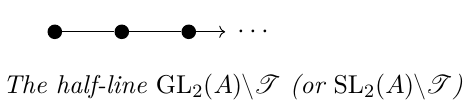
\includegraphics[scale=0.5]{halfline.png}
			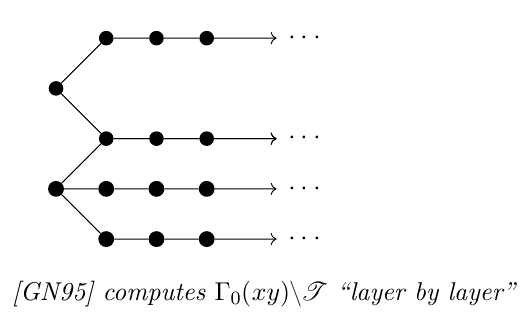
\includegraphics[scale=0.5]{layers.png}
			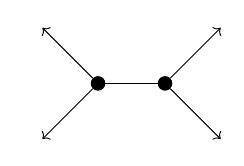
\includegraphics[scale=0.5]{quotient.png}\\
			We can ``read off'' that $\sX_{\Gamma_0(xy)}$ has $4$ cusps.
		\end{example}
	\end{frame}	
	
	\begin{frame}
		\frametitle{Cusps are Elliptic Points}
		\begin{columns} 
			% Column 1
			\begin{column}{.5\textwidth}
				Let $\Gamma^1\leq \SL_2(\bbZ).$ Consider a cartoon of $\Gamma^1\setminus(\cH\cup\bbP^1(\bbQ))$:
				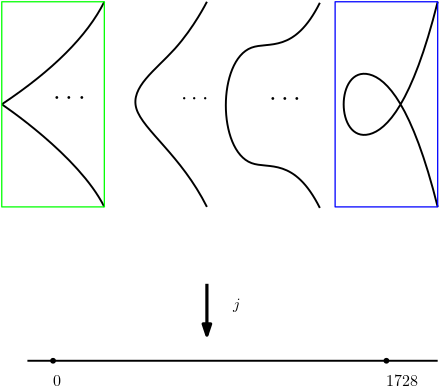
\includegraphics[scale=0.25]{ell.png}
				
				\pause
				\[\Gamma^1\setminus\bbP^1(\bbQ)\leftrightarrow\left(\begin{array}{c}\text{singular}\\\text{elliptic curves}\end{array}\right),\]
				but only elliptic curves with $j=0$ or $1728$ have extra automorphisms.
			\end{column}\pause
			% Column 2    
			\begin{column}{.5\textwidth}
				Let $\Gamma\leq \GL_2(A).$ Consider the moduli $\sX_{\Gamma}=[X_{\Gamma}/Z(GL_2(A))]:$ \pause
				\begin{align*}
					&\Aut(\varphi)\cong \bbF_q^{\times}& /\!/\bbF_q^{\times};\\ 
					&\Aut(\varphi_{(j=0)})\cong \bbF_{q^2}^{\times}& /\!/\bbF_q^{\times};\\ 
					&\Aut(\varphi_{(j=\infty)})\cong\{\begin{psmallmatrix}a&0\\0&d\end{psmallmatrix}\}&/\!/\bbF_q^{\times};
				\end{align*}
				so cusps on a stacky Drinfeld modular curve are elliptic points!
				%\[\Gamma\setminus\bbP^1(K)\leftrightarrow \left(
				%\begin{array}{c}\text{Drinfeld modules}\\\varphi_T\cong TX+X^q\\\text{of rank }1\end{array}\right),\]
				%
				%\pause
				%
				%\begin{lemma}
				%	Let $s\in \Gamma\leq \bbP^1(K).$ Then the maps $z\mapsto \alpha z$ for $\alpha\in C^{\times}$ in
				%	\[\operatorname{Stab}_{\Gamma}(s)\approx \{\begin{psmallmatrix}a&b\\0&d\end{psmallmatrix}: b\in A; a,d\in \bbF_q^{\times}\}\]
				%	are ``extra automorphisms'' of the associated rank $1$ D-module $\varphi_T.$
				%\end{lemma}
				%\begin{proof}
				%	All rank $1$ $C$-lattices are homothetic.\\
				%\end{proof}
				
			\end{column}
		\end{columns}
	\end{frame}
	
	\begin{frame}
		\frametitle{Elliptic Points on Stacky Curves}
		\begin{columns}
			\begin{column}{.5\textwidth}
				\begin{example}[Classical $j$-line]
					\begin{itemize}
						\item[$\cdot$] $X(1)=\SL_2(\bbZ)\setminus(\cH\cup\bbP^1(\bbQ))$ - the ``usual'' $j$-line $\bbP^1(\bbC)$ \pause
						\item[$\cdot$] $\overline{\cM_{1,1}}$ - DM stack representing the moduli of stable elliptic curves\pause
					\end{itemize}
					$\overline{\cM_{1,1}}$ is a $\mu_{2}$-gerbe over $\sX(1)=[X(1)/Z(\SL_2(\bbZ))],$ \pause i.e.\ $\sX(1)$ is a rigidification $\overline{\cM_{1,1}}/\!/\mu_{2}$: \pause
					\[\overline{\cM_{1,1}}\overset{\pi}{\to}\sX(1)\to X(1)\] \pause
					\[\begin{array}{ll}
						\bbP^1(4,6)\overset{\pi}{\to}\bbP^1(2,3)\to \bbP^1(\bbC)\end{array}.\]
				\end{example}
				
				%\begin{example}[{\cite[Remark $6.2.5$]{VZB}}]
				%	\begin{itemize}
				%		\item[$\cdot$] $\Gamma_0^1(N)\leq \PSL_2(\bbZ)$ - a typical congruence subgroup ($N\geq 1$) \pause
				%		\item[$\cdot$] $X^1_0(N) = \Gamma^1_0(N)\setminus(\cH\cup \bbP^1(\bbQ))$ - moduli of elliptic curves with cyclic $N$-isogeny \pause
				%		\item[$\cdot$] $\cM_0(N)$ - Deligne-Mumford stack representing the moduli problem \pause
				%	\end{itemize}
				%	The stacky modular curve $\sX_0^1(N)$ is a rigidification $\cM_0(N)/\!/\mu_{2}$ of the gerbe $\cM_0(N)$: \pause
				%	\[\cM_0(N)\overset{\pi}{\to}\sX_0^1(N)\to X_0^1(N)\]
				%\end{example}
			\end{column}
			\pause
			\begin{column}{.5\textwidth}
				\begin{example}[Drinfeld $j$-line]
					\begin{itemize}
						\item[$\cdot$] $X(1)=\GL_2(A)\setminus(\Omega\cup\bbP^1(K))$ - the ``usual'' $j$-line $\bbP^1(C)$ \pause
						\item[$\cdot$] $\cM^2_A$ - DM stack representing the moduli of rank $2$ Drinfeld modules with no level structure \pause
					\end{itemize}
					$\cM^2_A$ is a $\mu_{q-1}$-gerbe over $\sX(1)=[X(1)/Z(\GL_2(A))],$ \pause i.e.\ $\sX(1)$ is a rigidification $\cM^2_A/\!/\mu_{q-1}$: \pause
					\[\cM^2_A\overset{\pi}{\to}\sX(1)\to X(1)\] \pause
					\[\begin{array}{ll}
					\bbP^1((q-1)^2,q^2-1)\overset{\pi}{\to}\\\to\bbP^1(q-1,q+1)\to \bbP^1(C)\end{array}.\]
				\end{example}
			\end{column}
		\end{columns}
	\end{frame}
	
	\begin{frame}
		\frametitle{Rigid Stacky GAGA}
		
		\begin{theorem} Let $A$ be a $k$-affinoid algebra, for $k$ some non-achimedean field. 
		\begin{itemize}
			\item[](\cite[Lemma $7.2$]{Porta-Yu-Higher-analytic-stacks-GAGA}) Let $\sX$ be an algebraic stack locally of finite presentation over $\Spec(A).$ Suppose that for $\cF\in \cO_{\sX}-\operatorname{Mod}$ we have 
			\[\cF\cong\lim_{\tau\geq -n} \cF.\]
			Then the \textbf{analytification functor $(-)^{\text{an}}$} commutes with this limit. 
			
			\pause
			
			\item[](\cite[Theorems $7.4$ and $7.5$]{Porta-Yu-Higher-analytic-stacks-GAGA}) Let $\sX$ be a proper algebraic stack over $\Spec(A).$ \pause The analytification functor on coherent sheaves induces an equivalence of categories \pause
			\[\operatorname{Coh}(\sX)\overset{\cong}{\to} \operatorname{Coh}(\sX^{\text{an}}).\] 
			
			%\pause
			%
			%\item[](\cite[$7.3$]{Porta-Yu-Higher-analytic-stacks-GAGA}) Let $\sX$ be an algebraic stack locally of finite presentation/$\Spec(A).$ Suppose that $\cF,\cG\in\operatorname{Coh}(\sX).$ \pause There is an equivalence of categories given by the natural map \pause
			%\[\operatorname{Map}_{\operatorname{Coh}(\sX)}(\cF,\cG)\overset{\cong}{\to} \operatorname{Map}_{\operatorname{Coh}(\sX^{\text{an}})}(\cF^{\text{an}},\cG^{\text{an}}).\]
		\end{itemize}
		\end{theorem}
	\end{frame}
	
	\begin{frame}
		\frametitle{Geometry of Drinfeld Modular Forms $(1/3)$}
		\begin{columns} 
			% Column 1
			\begin{column}{.5\textwidth}
				Let $q$ be odd;\\
				Let $\Gamma\leq \GL_2(A)$;\\ 
				Let $\Gamma_2=\{\gamma\in \Gamma:\det(\gamma)\in (\bbF_q^{\times})^2\}.$ \pause\\
				Consider the cover of modular curves
				\begin{figure}[!h]\centering
					\begin{tikzcd}
						\sX_{\Gamma_2}\arrow[d]\\
						\sX_{\Gamma}
					\end{tikzcd}
				\end{figure}\pause
				When we compute the log canonical ring $R(\sX_{\Gamma_2}; 2\Delta)$ we get the following result.
			\end{column}\pause
			% Column 2    
			\begin{column}{.5\textwidth}
				\begin{theorem}[{\cite[$6.1$]{Franklin-geometry-Drinfeld-modular-forms}}]
					There is an isomorphism of graded rings \[M(\Gamma_2)\cong R(\sX_{\Gamma_2};\Omega^1_{\sX_{\Gamma_2}}(2\Delta)),\]\pause
					given by isomorphisms \[M_{k,l}(\Gamma_2)\to H^0(\sX_{\Gamma_2},\Omega^1_{\sX_{\Gamma_2}}(2\Delta)^{\otimes k/2})\] of form $f\mapsto f(dz)^{\otimes k/2},$ \pause where \\$k\equiv 2l\pmod{q-1}.$ 
				\end{theorem}
			\end{column}
		\end{columns}
	\end{frame}
	
	\begin{frame}
		\frametitle{Geometry of Drinfeld Modular Forms $(2/3)$}
		\begin{columns} 
			% Column 1
			\begin{column}{.5\textwidth}
				Let $q$ be odd;\\
				Let $\Gamma\leq \GL_2(A)$;\\ 
				Let $\Gamma_2=\{\gamma\in \Gamma:\det(\gamma)\in (\bbF_q^{\times})^2\}.$\\
				Consider the cover of modular curves\\
				\begin{figure}[!h]\centering
					\begin{tikzcd}
						\sX_{\Gamma_2}\arrow[d]\\
						\sX_{\Gamma}
					\end{tikzcd}
				\end{figure}\pause
				When we compare the modular forms for $\Gamma$ and $\Gamma_2$ we find the following.
			\end{column}\pause
			% Column 2    
			\begin{column}{.5\textwidth}
				\begin{theorem}[{\cite[$6.2$]{Franklin-geometry-Drinfeld-modular-forms}}]
					We have $M(\Gamma)\cong M(\Gamma_2),$ \pause
					with \[M_{k,l}(\Gamma_2)=M_{k,l_1}(\Gamma)\oplus M_{k,l_2}(\Gamma)\] on each component,\pause where $l_1,l_2$ are the solutions to $k\equiv 2l\pmod{q-1}.$ 
				\end{theorem}
			\end{column}
		\end{columns}
	\end{frame}	
	
	\begin{frame}
		\frametitle{Geometry of Drinfeld Modular Forms $(3/3)$}
		\begin{columns} 
			% Column 1
			\begin{column}{.5\textwidth}
				Let $q$ be odd;\\
				Let $\Gamma\leq \GL_2(A)$;\\ 
				Let $\Gamma_1=\{\gamma\in \Gamma:\det(\gamma)=1\}.$\\
				Suppose that $\Gamma_1\leq \Gamma'\leq \Gamma.$ \pause \\
				Consider the cover of modular curves
				\begin{figure}[!h]\centering
					\begin{tikzcd}
						\sX_{\Gamma'}\arrow[d]\\
						\sX_{\Gamma}
					\end{tikzcd}
				\end{figure}\pause
				When we compare the modular forms for $\Gamma$ and $\Gamma'$ we find the following generalization of \cite[Theorem $6.2$]{Franklin-geometry-Drinfeld-modular-forms}.
			\end{column}\pause
			% Column 2    
			\begin{column}{.5\textwidth}
				\begin{theorem}[{\cite[$6.12$]{Franklin-geometry-Drinfeld-modular-forms}}]
					We have $M(\Gamma)\cong M(\Gamma'),$ \pause
					and each component $M_{k,l}(\Gamma')$ is some direct sum of components $M_{k,l'}(\Gamma)$ for some nontrivial $l'.$
				\end{theorem}
			\end{column}
		\end{columns}	
	\end{frame}
	
	\begin{frame}
		\frametitle{Conclusion}
		\centering
		Thank you!\\ \pause 
		
		$~$\\
		
		Further details available at \href{https://arxiv.org/abs/2310.19623}{arXiv:$2310.19623$}\\
		
		$~$\\
		
		or in my thesis, which is available upon request. 
	\end{frame}
	
	\begin{frame}[allowframebreaks]
		\frametitle{References}
		\bibliography{bibliography}
		\bibliographystyle{amsalpha}
	\end{frame}
	
	
\end{document}